%\documentclass{article}
\documentclass[conference]{IEEEtran}
\IEEEoverridecommandlockouts
% The preceding line is only needed to identify funding in the first footnote. If that is unneeded, please comment it out.
\usepackage{cite}
\usepackage{amssymb,amsfonts}
\usepackage{algorithmic}
\usepackage{textcomp}
\usepackage[utf8]{inputenc}
\usepackage{amsmath}
\usepackage{graphicx}
\usepackage{xcolor}
\usepackage{accents}
\usepackage{array}
\usepackage{balance}
\usepackage{enumitem}
\setlist[itemize]{leftmargin=4.99mm}
%\usepackage[
%backend=biber,
%style=apa,
%citestyle=apa
%]{biblatex}

%\addbibresource{bibliography.bib} %Imports bibliography file
\begin{document}

%\title{User-centric and Context-aware  Recommender System for e-Tourism}

\title{User-centric and Context-aware  Recommender System for e-Tourism}


\author{\IEEEauthorblockN{Gustavo Castellanos}
\IEEEauthorblockA{\textit{Computer Science Department} \\
\textit{Universidad Simón Bolívar}\\
Caracas, Venezuela \\
14-10192@usb.ve}
\and
\IEEEauthorblockN{Yudith Cardinale}
\IEEEauthorblockA{\textit{Computer Science Department} \\
\textit{Universidad Simón Bolívar}\\
Caracas, Venezuela \\
ycardinale@usb.ve}
\and
\IEEEauthorblockN{Philippe Roose}
\IEEEauthorblockA{\textit{Université de Pau et des Pays de l’Adour} \\
\textit{LIUPPA -- T2I64600}\\
Anglet, France \\
philippe.roose@iutbayonne.univ-pau.fr}
%\and
%\IEEEauthorblockN{Yudith Cardinale}
%\IEEEauthorblockA{\textit{Computer Science Department} \\
%\textit{Universidad Simón Bolívar}\\
%Caracas, Venezuela \\
%ycardinale@usb.ve}
%\and
%\IEEEauthorblockN{Marc Dalmau}
%\IEEEauthorblockA{\textit{Université de Pau et des Pays de l’Adour} \\
%\textit{LIUPPA -- T2I64600}\\
%Anglet, France \\
%dalmau@iutbayonne.univ-pau.fr}
%\and
%\IEEEauthorblockN{Nadine Couture}
%\IEEEauthorblockA{\textit{ESTIA Technopole Izarbel} \\
%\textit{64210}\\
%Bidart, France \\
%n.couture@estia.fr}
%\and
%\IEEEauthorblockN{Dominique Masson}
%\IEEEauthorblockA{\textit{dept. name of organization (of Aff.)} \\
%\textit{name of organization (of Aff.)}\\
%City, Country \\
%email address or ORCID}
}


%\author{Gustavo Castellanos and Yudith Cardinale and Philippe Roose }
%\date{November 2019}


\maketitle

\begin{abstract}
Often travelers try to manually collect enough information for planing to go to a destination, but this task may be overwhelming due to the big amount of options. Usually, tourists depend on places' reviews to make the choice, but this implies prior knowledge of the existence of the places. These reviews are often requested on tourism sites and applications, most of which follow the PULL paradigm, i.e., the user has to explicitly search for suggestions/recommendations through interaction with the application's graphical user interface. On the other hand, a
PUSH approach, in which the application proactively triggers a recommendation process when
necessary (for example, when the user is close to a POI, when lunch time is approaching, or
when weather conditions change) seems to be a more reasonable solution. Having said that, in this work we propose a user-centric hybrid recommender system, using an ontology-based algorithm for content-based and context-aware recommendations, with a focus on decreasing predictable output under same situations, i.e., increasing serendipity. To demonstrate its suitability and performance, we test it in different simulated scenarios using different weights or priorities for the predicted preferences, context activations, aging and distances of the recommended places.
\end{abstract}
\begin{IEEEkeywords}
tourism, recommender systems, context awareness
\end{IEEEkeywords}


\section{Introduction}
%\textcolor{red}{XXXLa intro y el abstract deben tener la siguiente estructura: hablar del contexto general: Turismo y e-tourismo dado los avances tecnológicos; lo que se usa y sus limitaciones (que es el párrafo que tienes ahora); luego lo que se propone (la contribución del paper, la conclusión general de los resultados y finalmente la organización del paperXXXX}

%\textcolor{red}{XXX Pondré en rojo XXXXMis comentariosXXXXXXXX y los párrafos que redacte/cambie. Así los ubicas más fácilmente}

Tourism is one of the most promising areas for diverse applications and is becoming an extremely
important market \cite{buhalis2011tourism,murphy2013tourism,fermoso2015open,ku2015cultivating,alghamdi2016tourism,artemenko2017tourism,kazandzhieva2019tourism}. 
When travellers are going or planning to go to a destination, they try to collect information about their new destination “as best they can” (e.g., by going to the tourist office or by obtaining information about their destination and its surroundings on the Internet). Usually, tourists depend on places' reviews to decide where to spend their vacations, their free time, or even their lunch or just their afternoon, but this requires prior knowledge of the existence of the places. Furthermore, sometimes people know about a place but do not know if it is a good fit for their necessities and ignores it, taking the risk of missing a good experience. Nevertheless, this requires a considerable amount of effort on the part of the tourists.

Currently, there is a plethora of applications offering information on cities and historical centres, points of interest (POIs) to visit, city tours, green areas to rest, etc. The use of such applications implies that the user is first aware of them, then installs them in the hope that they are suitable (only 10\% of downloaded mobile applications are used more than once), learns and knows how
to use them and then filters the data/information that is uploaded or offered. Most of these
applications follow the PULL paradigm, i.e., the user has to explicitly search for
suggestions/recommendations through interaction with the application’s graphical user interface.
We believe that this is one of the reasons why these types of applications are not successful: they
require too many steps, too many interactions, and too many unknowns. On the other hand, a
PUSH approach, in which the application proactively triggers a recommendation process when
necessary (for example, when the user is close to a POI, when lunch time is approaching, or
when weather conditions change) seems to be a more reasonable solution. A first step in this
direction has been taken by Google via Google Now\footnote{https://www.google.com/intl/fr/landing/now/}, 
which provides information/suggestions
to users by detecting in their geographical environment what they need according to their
location and time. However, such applications are simplistic and use only a limited amount of
information, and moreover, do not take into account the user’s activity. A key element is the
consideration of the users' context, such as their locations, weather (\textit{is it raining?}), or time (\textit{is it night?}).

Recommender Systems are now at the heart of
much research and offer real benefits to users, organizations, and the business community in
general~\cite{borras2014intelligent,del2016pull,leskovec2020mining}. In the context of tourism, most recommender systems are able to predict user's preferences based on previous activities, but research on Context-Aware Recommender Systems
(CARS) are still to be further developed~\cite{adomavicius2011context,nejma2015service,haruna2017context,raza2019progress}. Additionally, most recommender systems do not consider to vary the recommendations -- i.e., they become predictable  for same users, under the same situations. Thus, there is still a real need for research and design of innovative solutions in this field. Nowadays, the use of ontologies to represent the knowledge related to tourism (POI, users' information, context information, etc.) is becoming a powerful tool to offer such as innovative solutions \cite{rajaonarivo2019rec} \cite{bahramian_abbaspour_claramunt_2017}, being DATATourisme\footnote{http://info.datatourisme.gouv.fr/ontology/core/2.0/} a good example.

In this context, in this work we propose a user-centric hybrid recommender system, using an ontology-based algorithm for serendipious content-based and context-aware recommendations. According to the users’ wishes, the serendipity of recommendations may increase (e.g., surprise events, unrepeated recommendations)~\cite{kotkov2016survey}. All this based on an {\it aging}-like algorithm, which gives less priority to recently recommended places.  It is also desirable that the user knows why something is recommended (i.e., that the recommendations are explainable). We describe the architecture and algorithms of our recommender system. To demonstrate its suitability and performance, we test it in different simulated scenarios using different weights or priorities for the predicted preferences, context activations, aging and distances of the recommended places.

We organize the rest of this paper as follows. In Section \ref{section:related-work}, we survey 
%introduces 
relevant studies related to our work.
%and concepts for understanding our system. 
Section \ref{sec:proposal} describes the architecture and functioning of our proposed system. Section \ref{section:study-case} describes results obtained during the experiments. Finally, Section \ref{section:conclu} explains our final thoughts.



\vspace{-0.2cm}
\section{Related Work} \label{section:related-work}

% \textcolor{red}{Clasificar los sistemas de recomedación de acuerdo a: User-centric (manual, automatic); context-aware; ontology-based; used methods (ML, DL, heurísticas, modelos, etc.)\\
% INCLUIR (y otros):\\

% - Efficient user profiling based intelligent travel recommender system for individual and group of users, 2019 NO PDF\\
% - Ingrid Christensen, Silvia Schiaffino, and Marcelo Armentano.Social group recommendation in the tourism domain. Journal of intelligent information systems, 47(2):209–231, 2016\\ NO PDF
% - L Rizaldy Hafid Arigi, Z K Abdurahman Baizal, and Anisa Herdiani. Context-aware recommender system based on ontology for recommending tourist destinations at bandung. Journal ofPhysics: Conference Series, 971:012024, mar 2018. } NO PDF

%\subsection{Recommender Systems} %\label{section:recommender-systems}

The unleashed proliferation  of recommender systems for tourism domain, due to the current development of mobile Internet technology, has fostered a wide categorization of them. 
Depending on the technique used to 
%resolve 
make recommendations, these systems are %usually 
classified into two categories: memory-based and model-based~\cite{bobadilla2013recommender,ebrahim_2012}. \textbf{Memory-based} recommender systems support their  suggestions on similarities among users and their shared items, hence recommending similar items to the ones the user likes (i.e., \textit{content-based recommendation}) or recommending items liked by users that are similar to the user (i.e., \textit{collaborative filtering}). \textbf{Model-based} recommender systems try to guess how much a user will like an item that they did not consume before, usually through statistical techniques and machine-learning models. Recommender systems that combine both 
%memory-based and model-based 
approaches are called \textbf{Hybrid} recommender systems.

%In this section, 
We survey some relevant and recent studies in the tourism domain, classifying them according to these three categories and considering aspects related to  how they manage users' preferences and interests, the context awareness, the use of ontologies, and the variability of recommendations. We compare %the related work 
them in terms of these criteria and highlight the difference with our proposal.    

\vspace{-0.3cm}
\subsection{User information}
%Obviously, 
All recommender systems take into account some information related to the user, such as identification aspects (sex, age, profession, etc.), interest and preferences, or social relations. This information can be explicitly (e.g., questionnaires)~\cite{jannach2020interactive} or implicitly (e.g., by analyzing feedbacks in user's social networks)~\cite{lin2018hybrid} obtained.  
%This information can be obtained from explicit (e.g., questionnaires)~\cite{jannach2020interactive} or implicit (e.g., by analyzing feedbacks in user's social networks) media~\cite{lin2018hybrid}.  

Some proposals are supported on users' interaction to obtain their data (i.e., following a PULL paradigm). In  %Rajaonarivo et al.
~\cite{rajaonarivo2019rec}, authors model the users' information considering their gender, age category (e.g., kid, adult, or elderly), and preferences, classified as thematic preferences (e.g., museum, theater) and historical preferences (e.g., 12th century), that have to be provided by them through a user interface.  In~\cite{santos2019using}, only health,  physical, and psychological conditions are required  with forms filled by users. 
Users' preferences and feedback are directly assigned by the users in the proposal presented in~\cite{bahramian_abbaspour_claramunt_2017}. As in ~\cite{arigi2018context}, users' interest (i.e., not interested, less interested, and interested enoughd) on tourism categories are asked to them. SMARTMUSEUM~\cite{ruotsalo2013smartmuseum}, asks users about the desired duration of a visit to a particular location, the motivation for a visit, and ability to consume the content offered by the system. The system proposed in~\cite{shen2016attraction} requires photos uploaded by users, from which it extracts their travel history; it also asks users to rank  POI (their favorite and non-favorite attractions).
 

Other recommender systems extract users' information, mainly their preferences and interests, from available sources,
without asking for explicit interaction.  The work presented in~\cite{kesorn2017personalized}, takes from Facebook basic information (e.g., name, age) and  check-in data (e.g., visited places)  to identify users' interests and preferences. 
To automatically deduce users' preferences from their social networks, many techniques are used, such as opinion mining~\cite{logesh2019exploring,logesh2018personalised}, analysis of implicit/explicit feedback~\cite{hidasi2016general}, and analyzing geotagged pictures~\cite{sun2019building}. 
Curumim~\cite{menk2017curumim} takes from users' social networks their travel history and level of education, and predicts their degree of curiosity. Most of these works follow the PULL approach.


Many other proposals combine both explicit and implicit users' information gathering, also under the PULL paradigm. SPETA~\cite{garcia2009speta},  supports  its recommendation on the interest and rating  of tourism places that users explicitly provide, and on preferences deduced by analyzing their behavior on social networks. The system presented in~\cite{alonso2012ontology}, takes into account special needs and  context-dependent preferences on tourism sites, directly  provided by users, as well as explicit/implicit feedback on their social networks. 

\vspace{-0.4cm}
\subsection{Context-awareness}
In order to improve suggestions, the trend is to consider context aspects that describe a specif situation in a determined moment for a user, including transportation media, weather, time, or even health conditions. Many works use context-modeling approaches that mainly consider means of transportation, travel time,  location, or weather~\cite{rajaonarivo2019rec,bahramian_abbaspour_claramunt_2017,arigi2018context,kesorn2017personalized,logesh2019exploring,logesh2018personalised}.


SMARTMUSEUM~\cite{ruotsalo2013smartmuseum} only considers users' location as contextual information captured by the built-in sensors of mobile devices, such as GPS, accelerometers, and RFID readers. The system proposed in~\cite{shen2016attraction} collects automatically the users' current location (city, latitude, and longitude) and current time, thus recommendations are influenced by the geo-distance to POI. SPETA~\cite{garcia2009speta} also considers users' location extracted from users' mobile devices, but it takes into account current and the history of past locations. It also gathers from  mobile devices other contextual information, such as weather forecast and time. 


A General Factorization Framework for context-aware recommender systems is proposed in~\cite{hidasi2016general}, with the aim of constructing factorization matrices (not matter which and how many context factors are considered) for machine learning techniques. In~\cite{sun2019building}, it is used a combination of contextual information like weather, transportation, or textual information, with geotagged pictures taken by the user for building the user model.
The system proposed in~\cite{alonso2012ontology}, is the only one among the referenced works that considers context-dependent   preferences, as our proposal,  related to weather, day, transport, and special needs. It means that users' preferences for POI, are expressed with regards the context (e.g., {\it indoor places when is raining}, {\it art exhibitions at night}).


%The work proposed in~\cite{rajaonarivo2019rec},
%Rajaonarivo et al.
% uses a
%context-modeling approach that considers means of transportation, travel time, and location. LISTO

%Kesorn et al. \cite{kesorn2017personalized} use the time of the day for achieving more suitable recommendations. LISTO

%The system proposed in~\cite{alonso2012ontology}, is the only one among the referenced works that considers context-dependent   preferences, as our proposal,  related to weather, day, transport, and special needs. It means that users' preferences for POI, are expressed with regards the context (e.g., {\it indoor places when is raining}, {\it art exhibitions at night}).


%Logest et al. \cite{logesh2019exploring} \cite{logesh2018personalised} also consider user context like user location.  LISRO


%Bahmarian et al. \cite{bahramian_abbaspour_claramunt_2017} consider weather, time, and day. LISTO

\vspace{-0.2cm}
\subsection{Serendipity}

A useful goal for a recommender system is to be serendipitous, which 
%accordingly to Kotkov et al. \cite{kotkov2016survey} 
means that the recommended items must be relevant, novel, and unexpected. A relevant item is an item that the user likes, consumes, or is interested in; a novel item is one
%an item 
that users have never seen or heard about in their life; an unexpected item 
is 
%an item that 
significantly different from the profile of the user. Some quite good recent surveys emphasize the importance of such as feature for recommender systems in general~\cite{kotkov2016survey,chen2019serendipity} and in the tourism domain~\cite{tintarev2010off,menk2019recommendation}.

%The same work explains the differences between novelty and unexpectedness: "First, a user may find an item unexpected even if she/he is familiar with the item. Second, to surprise a user, unexpected items have to differ from the user profile more than novel items".

It starts to be a trend to recommend  POI. The model considered in~\cite{rajaonarivo2019rec}, considers previous activity of other users to recommend tours of POI, thus reducing overspecialization and increasing serendipity, however experiments with this feature were not made. Authors of~\cite{shen2016attraction} assert that the proposed system is able to recommend fresh and surprise POI, based on collective intelligence.
 From the level of curiosity predicted from users' social networks, Curumim~\cite{menk2017curumim}  adapts the degree of surprise and unexpectedness of a recommended POI, tailored to users' curiosity values. 






%Rajaonarivo et al. \cite{rajaonarivo2019rec} model considers previous activity of other users to recommend tours of POI, thus reducing overspecialization and increasing serendipity, however experiments with this feature were not made.
\vspace{-0.2cm}
\subsection{Use of ontologies}

The huge amount of data that can be managed in recommender systems, related to users' information, users' preferences, context factors, POI, etc.,   demands the use of more complex knowledge. Even though, recommender system is an area that has been the focus of many studies, thus reaching a very good level of maturity, there is still a lack of standardization to represent such information. In this sense, it is evident the necessity of a well-defined and standard model for representing the knowledge managed by recommender systems. Semantic Web, in particularly the use of ontologies, seems to be a clear solution, from which we can take its organizational and relational capacity.
In the context of tourism, ontology-based  recommender  system  is  an  emerging  trend~\cite{borras2014intelligent,yochum2020linked}.

Some systems only count on ontologies to represent tourism  POI~\cite{rajaonarivo2019rec,bahramian_abbaspour_claramunt_2017,garcia2009speta,arigi2018context}. Other works consider user profile ontologies, besides tourism ontologies, such in~\cite{ruotsalo2013smartmuseum}. In~\cite{alonso2012ontology}, an ontology to represent user preferences and context factors is proposed.



%Rajaonarivo et al. \cite{rajaonarivo2019rec} export the data used to well known open data platforms before using it; 

%Bahmarian et al. 
%\cite{bahramian_abbaspour_claramunt_2017} based their proposal on spreading activation algorithms on the nodes of an e-tourism ontology.

\vspace{-0.2cm}
\subsection{Discussion}

Table \ref{table:related-work} shows a comparative evaluation  of the referenced works, in terms of \textbf{category} of the system (model-based, hybrid, etc.), type of \textbf{user's information} gathered, \textbf{context} factors considered, \textbf{ontology} used, and how they handle \textbf{serendipity}. 

Rajaonarivo et al. \cite{rajaonarivo2019rec} is the only work that proposes a context-aware system using ontologies and approaching serendipity, as our proposed system RECESO, nonetheless they did not experiment the serendipitous feature. In contrast, our work does evaluate the serendipity of our proposed system. Moreover, RECESO supports the PUSH paradigm by implicitly gathering users' preferences and context, and the PULL paradigm by explicit user interactions.

%Our work does evaluate the serendipity of our proposed system, which can support the PUSH paradigm by implicitly gathering users' preferences and context, and the PULL paradigm by explicit user interactions.

\begin{table*}[h!]
\footnotesize{
    \centering
    \caption{Related work on recommender systems for e-tourism}
    \label{table:related-work}
    \vspace{-0.3cm}
    \begin{tabular}{|c|c|c|c|c|c|} 
        \hline
        \textbf{Work} & \textbf{Category} & \textbf{Users' information} & \textbf{Context}&\textbf{Ontology}&\textbf{Serendipity} \\
        \hline \hline 

        \cite{rajaonarivo2019rec} & Hybrid & Basic, Preferences & Transportation, Location, Weather & Tourism & Collaborative \\ \hline

        \cite{santos2019using} & Model-based & Health & & & \\ \hline

        \cite{bahramian_abbaspour_claramunt_2017} & Hybrid & Preferences & Weather, Time, Day & Tourism, Context & \\ \hline

        \cite{arigi2018context} & Model-based & Preferences & Transportation, Location, Weather & Tourism & \\ \hline

        \cite{ruotsalo2013smartmuseum} & Model-based & Duration, Motivation, Ability & Location & Tourism, User & \\ \hline

        \cite{shen2016attraction} & Model-based & Preferences, travel history & Location, Time & & Surprise \\ \hline

        \cite{kesorn2017personalized} & Hybrid & Social, Check-in data & Transportation, Location, Weather & & \\ \hline

        \cite{logesh2019exploring} & Hybrid & Social, Opinion mining & Transportation, Location, Weather &  & \\ \hline

        \cite{logesh2018personalised} & Hybrid & Social, Opinion mining & Transportation, Location, Weather &  & \\ \hline

        \cite{hidasi2016general} & Model-based & Social, Feedback  & General &  & \\ \hline

        \cite{sun2019building} & Model-based & Social, Pictures & Transportation, Weather, Textual &  & \\ \hline

        \cite{menk2017curumim} & Hybrid & Social, History, Education &  &  & Curiosity \\ \hline

        \cite{garcia2009speta} & Hybrid & Preferences, Social & Location & Tourism & \\ \hline

        \cite{alonso2012ontology} & Hybrid & Social, Preferences & Weather, Day, Transport, Special Needs & Tourism, Context & \\ \hline

        \hline
        RECESO & Hybrid & Preferences & Weather, Time, Day, Location & Tourism & Aging \\ \hline

        \hline
    \end{tabular}
    \vspace{-0.3cm}
    }
    \end{table*}


% \subsection{Usage of ontologies: Spreading Activation} \label{section:usage-spreading-activation}
% Previous work \cite{bahramian_abbaspour_claramunt_2017} integrates the concepts of recommender systems with ontologies at building a context-aware tourism recommender system based on the \textit{spreading activation} algorithm. In its authors' own words: "In spreading activation method, a given concept is represented by a node and has an activation value. A relation among different concepts is represented by a link between nodes and has a weight value. To initialize the algorithm, one or several nodes of a network are activated and these activations spread to the relevant nodes. This process is iterated until a stopping condition (e.g., number of node processed) is reached". The activation value of the node \(v_i\) is computed as follows:
% \begin{equation} \label{eq:og_activation}
% a_{v_i} = \sum_{v_j \in neighbors(v_i)} w_{v_i, v_j} a_{v_j} 
% \end{equation}
% where $a_{v_i}$ is the activation value of node $v_i$, $neighbors(v_i)$ is the set of $v_i$'s neighbor nodes and $w_{v_i, v_j}$ is the weight of the link between $v_i$ and $v_j$. This concept will be useful in further sections. 

% \subsubsection{Semantic Network}
% Behmarian et al. \cite{bahramian_abbaspour_claramunt_2017} extend the information available for a tourism ontology so it can be used with spreading activation algorithm. A \textit{preference} and a \textit{confidence} values are associated to each ontology class. Each link has a weight that represents the degree of relationship between two classes or concepts. An ontology of different context scenarios or \textit{context factors} is linked to the tourism ontology, where the context factors are related to distance to POIs, time and weather information. The activation values of the nodes of the context ontology represent the level of fulfillment based on some measurement. The extended ontology is called \textbf{semantic network}.

% \subsubsection{Learning Phase}
% Bahmarian et al. \cite{bahramian_abbaspour_claramunt_2017} defined the \textit{preference} and the \textit{confidence} for an ontology class $c$ during learning phase as follows:

% \begin{equation} \label{eq:preference}
%     pref_c = \frac{\displaystyle \sum_{p \in ancestors(c)}{conf_p pref_p}}
%                     {\displaystyle  \sum_{p \in ancestors(c)} {conf_p}}
% \end{equation}

% \begin{equation} \label{eq:confidence}
%     conf_c = \frac{\displaystyle \sum_{p \in ancestors(c)} {conf_p}}{|ancestors(c)|} - \alpha
% \end{equation}
% where $ancestors(c)$ is the set of ancestors of the ontology class $c$, $pref_c$ is the preference of the class $c$, $conf_c$ is the confidence of the class $c$ and $\alpha$ is the \textit{decrease rate} that will tell how much should decrease the \textit{confidence} at each level. These formulas are applied to each node traversing from the root or sources.

% \subsubsection{Recommendation Phase}
% To contextualize the recommendation, "\textit{the context factors are used as initial nodes in the spreading activation and transmit the activation flow}" \cite{bahramian_abbaspour_claramunt_2017}, then the activated nodes are recommended. 

% The feature of using sets of similar items without using statistical models such as clustering but using ontology classes, and also predicting the user preferences, makes this kind of systems to be hybrid recommender systems.

% \subsection{Serendipity} \label{section:serendipity}
% An useful goal for a recommender system is to be serendipitous, which accordingly to Kotkov et al. \cite{kotkov2016survey} means that the recommended items must be relevant, novel and unexpected. A relevant item is an item that the user likes, consumes or is interested in; a novel item is an item that the user has never seen or heard about in their life; an unexpected item is an item that significantly differ from the profile of the user. The same work explains the differences between novelty and unexpectedness: "First, a user may find an item unexpected even if she/he is familiar with the item. Second, to surprise a user, unexpected items have to differ from the user profile more than novel items.".

% Kotkov et al. \cite{kotkov2016survey} define many ways to measure how serendipitous a recommender system is, through measuring first relevance, novelty and unexpectedness of its recommendations. Since a recommender system will probably predict the preference a user has for a specific item, hence predict the relevance of the item, we are mainly focused on novelty and unexpectedness.

% There is a metric proposed by Nakatsuji et al. (as cited in \cite{kotkov2016survey}) for novelty that uses the taxonomy classes to which each recommended item belongs and their distance between them, being the minimum distance of a new recommended item $i$ to each already recommended item $j$ the novelty of the item $i$:
% \begin{equation}
%     nov_{na}(i, u) = \underaccent{j \in I_u}{min}(dis(cls_j, cls_i))
% \end{equation}
% where $cls_k$ is a class of item $k$ in the taxonomy and $dis(cls_j, cls_i)$ is the distance between classes $cls_j$ and $cls_i$ in the taxonomy. Since our work is focused on the use of an ontology on tourism field, this metric is very helpful.

% % \subsection{Ontologies for e-tourism algorithm}

\section{Our Proposal}
\label{sec:proposal}

In this section we describe the architecture and functioning of our proposed User-Driven and Context-aware Hybrid Recommender System. Figure \ref{fig:arquitecture} shows its components:
\begin{itemize}
    \item \textbf{Data Gathering Module}: User preferences are received by the system, explicitly (direct interaction) or implicitly (data mining, social network analysis, etc.).
    \item \textbf{User Interest Module}: The preferences are propagated from higher classes to lower classes.
    \item \textbf{Context Module}: The system receives information about the context of the user, explicitly or implicitly (retrieved from an API, mobile information, etc.).
    \item \textbf{Recommendation Module}: The system recommends a set of places to the user.
\end{itemize}

In the following sections, we describe in detail each module.

\begin{figure}[h]
\centering
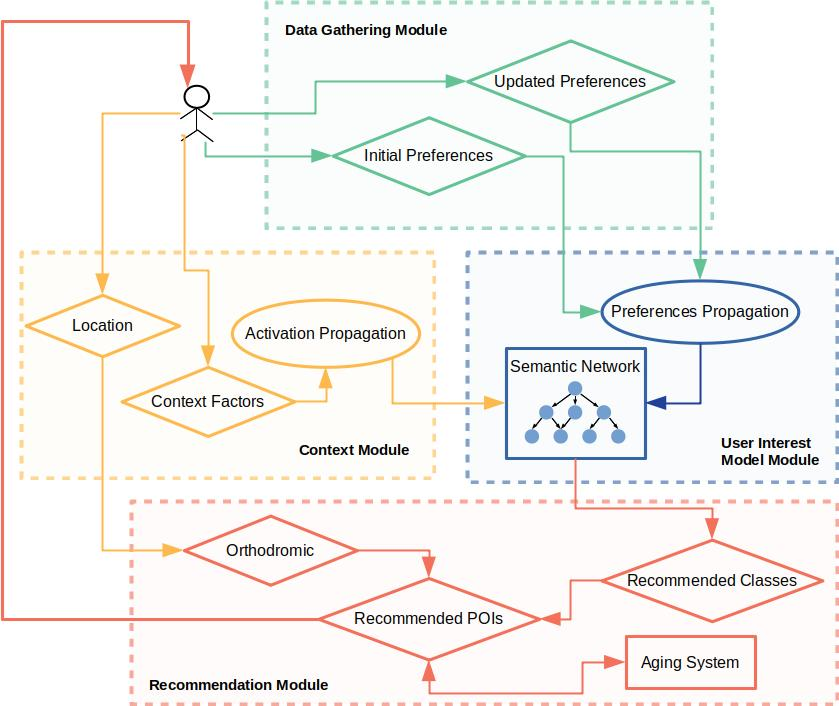
\includegraphics[scale=0.4]{draws/arquitecture.jpg}
\caption{System arquitecture}
\label{fig:arquitecture}
\end{figure}

\subsection{Data Gathering Module}
Initially, the system should receive initial \textbf{preferences}, as real values between $0$ and $1$, for the higher classes. To obtain these values, the user could explicitly set them by interacting with the system or they could be implicitly determined using data mining, social network analysis, geo-data, etc. During the lifetime of the system, the user can feed new updated preferences to the system.

\subsection{User Interest Model Module}
Inspired on the work of Bahramian et al. \cite{bahramian_abbaspour_claramunt_2017}, we introduce the concept of \textbf{semantic network}: a tourism ontology extended with the user's preferences (see figure \ref{fig:initial_pref}) and context factor links, a concept we explain later (see figure \ref{fig:init_act}). Just like Bahramian et al. \cite{bahramian_abbaspour_claramunt_2017}, we take advantage of the hierarchical shape of the semantic network for propagating the preference of superclasses to subclasses. Alongside preferences, each node of the semantic network has a \textbf{confidence} related to the user, a real value between $0$ and $1$ that defines how sure is the system that the computed preference is the real one. For computing the preference and the confidence we use formula \ref{eq:preference} and formula \ref{eq:confidence}, respectively:
\begin{equation} \label{eq:preference}
    pref_c = \frac{\displaystyle \sum_{p \in ancestors(c)}{conf_p pref_p}}
    {\displaystyle  \sum_{p \in ancestors(c)} {conf_p}}
\end{equation}
\begin{equation} \label{eq:confidence}
    conf_c = \frac{\displaystyle \sum_{p \in ancestors(c)} {conf_p}}{|ancestors(c)|} - \alpha
\end{equation}
where $ancestors(c)$ is the set of ancestors of the ontology class $c$, $pref_c$ is the preference of the class $c$, $conf_c$ is the confidence of the class $c$ and $\alpha$ is the \textit{decrease rate} that will tell how much should decrease the \textit{confidence} at each level. 

These formulas are applied to each node traversing from the higher classes, whose preferences are obtained from the Data Gathering Module, to the leaves. This process is called \textbf{preference propagation} and figures \ref{fig:initial_pref} and \ref{fig:pref_prop} show an example.

\begin{figure}[h]
\centering
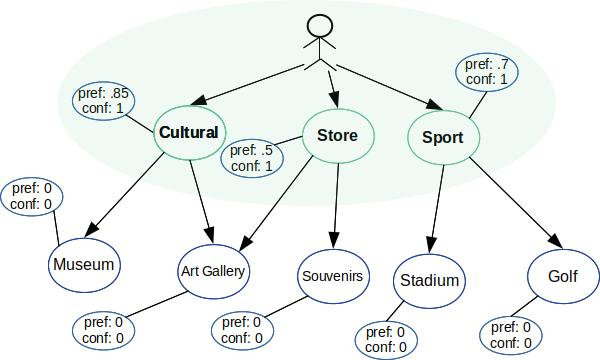
\includegraphics[scale=0.5]{draws/initial_pref.jpg}
\caption{Initial preferences for "Cultural", "Store" and "Sport" classes}
\label{fig:initial_pref}
\end{figure}

\begin{figure}[h]
\centering
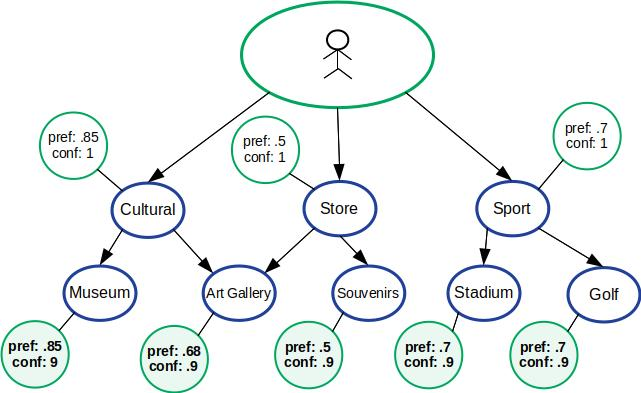
\includegraphics[scale=0.5]{draws/pref_spred.jpg}
\caption{Preference propagation for "Museum", "Art Gallery", "Souvenirs", "Stadium" and "Golf" classes, with decrease rate equal to 0.1}
\label{fig:pref_prop}
\end{figure}

\subsection{Context Module}
We define the \textbf{activation} of a node as the value that determines how feasible it is to go to a place that belongs to the node's ontology class in the current user's context. The user's context is determined by the \textbf{context factors}, entities that describe the characteristics of the user’s context that could affect their decision to go to a specific place. The context factors could be time, day and weather, as proposed by Bahramian \cite{bahramian_abbaspour_claramunt_2017}, but many others could be used, like transportation\cite{rajaonarivo2019rec} and mood. These entities are linked to the higher classes.

Let's define $f_x$ the \textit{fulfillment} of a context factor $x$ that has the value $1$ if $x$ fulfills or $0$ otherwise. Let's also define $r_{c,x}$ as the \textit{relevance} of context factor $x$ for node $c$, which is a real value in $[0, 2]$ that specifies how much the context factor can affect the decision to go to a POI that belongs to the node's ontology class; a value of $1$ means indifference; a value near $2$ means the fulfillment increases the wish to go to the POI; a value near $0$ means the fulfillment decreases the wish to go the POI. Hence, we define the activation for a node whose class $c$ is directly linked to the context factors:
\begin{equation} \label{eq:high_activation}
    act_c = \sum_{x \in contextFactors} r_{c,x} f_x
\end{equation}
and the activation for the internal nodes is defined as follows:
\begin{equation} \label{eq:activation}
    act_c = \frac{\displaystyle \sum_{c' \in ancestors(c)} act_{c'}}{|ancestors(c)|}
\end{equation}.
These formulas are used for an \textbf{activation propagation} from the higher classes. Figures \ref{fig:init_act}, \ref{fig:high_act} and \ref{fig:spread_act} show an example.

\begin{figure}[h]
\centering
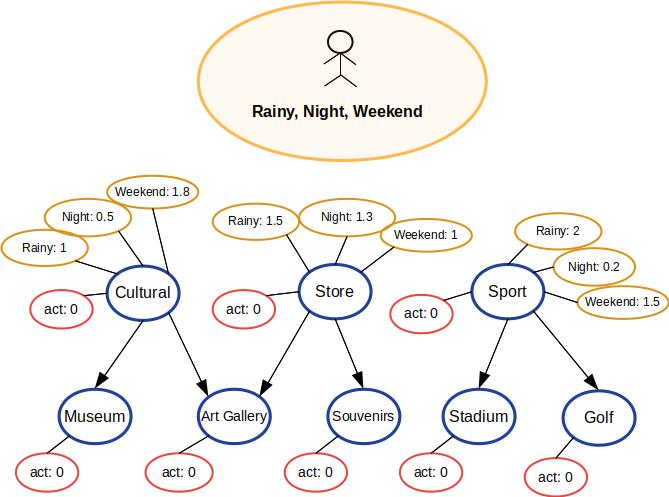
\includegraphics[scale=0.45]{draws/initial_act.jpg}
\caption{System receives (sunny, night, weekend) as user context}
\label{fig:init_act}
\end{figure}

\begin{figure}[h]
\centering
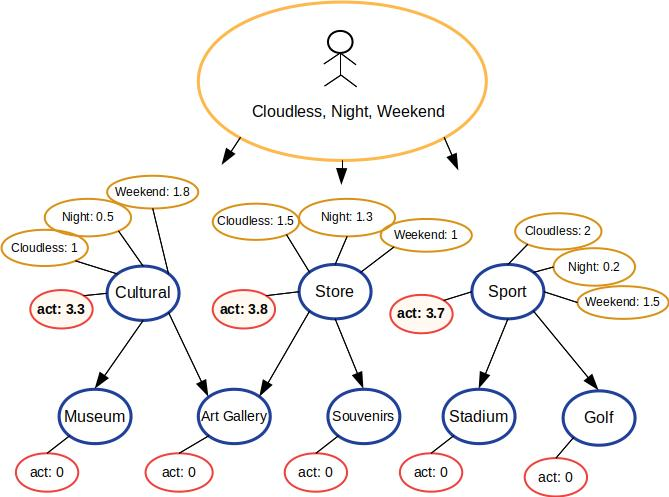
\includegraphics[scale=0.45]{draws/high_act.jpg}
\caption{Compute activation for "Cultural", "Store" and "Sport" classes}
\label{fig:high_act}
\end{figure}

\begin{figure}[h]
\centering
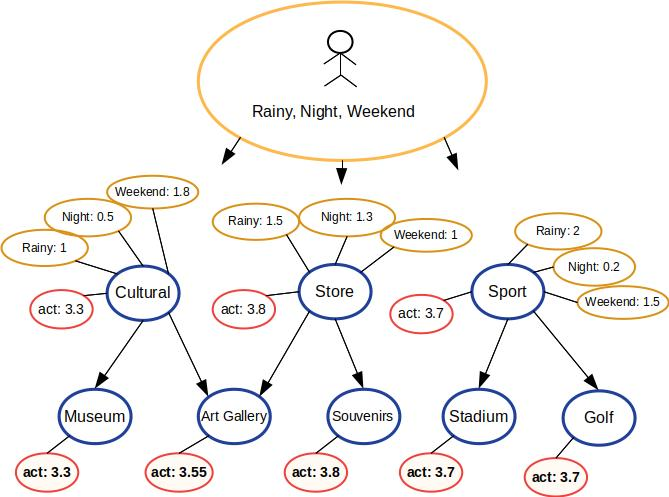
\includegraphics[scale=0.45]{draws/spread_act.jpg}
\caption{Spread activation to "Museum", "Art Gallery", "Souvenirs", "Stadium" and "Golf" classes}
\label{fig:spread_act}
\end{figure}

Furthermore, this module receives the user's \textbf{location}, which will be used for querying near POIs.

\subsection{Recommendation Module}

We will first give two necessary definitions to compute the final score of an item and then we give the formula.

\subsubsection{Aging System}

Let's define $\eta_p$ as the POI $p$'s aging, initialized on $\eta_p = 1$. Let's define $H$ as the \textit{aging rate}. Each time a POI $p$ is recommended to the user, $\eta_p$ decreases by $H$. When $\eta_p < 0.1$, $\eta_p$ is reset to $1$. 

\subsubsection{Great-Circle distance}
Since the euclidean distance between two points on Earth would cross through the surface, we should use a more convenient measurement of distance: the \textit{great-circle distance} or \textit{orthodromic distance}. It is the shortest distance, along the surface of a sphere, between two points on the surface of the sphere. It is measured with circles on the sphere whose centers coincide with the center of the sphere. Those circles are called \textit{great-circles}. If we assume Earth is a perfect sphere and hence use Great-Circle distance, we get distances with errors no more than $0.5\%$ according to \cite{1997admiralty}. 

The distance between two points $i$ and $j$ on a sphere of radius $r$ is computed with the following formula:
\begin{equation} \label{eq:gc-dist}
    \begin{split}
        \scriptstyle{dist_{i,j} \ = \ r \cdot arccos (} & \scriptstyle{cos(lat_i) \cdot cos(lat_j) \cdot cos(lon_i - lon_j)} \\
                                        & \scriptstyle{+ \ sin(lat_i) \cdot sin(lat_j) )}
    \end{split}
\end{equation}

\subsubsection{Score} \label{section:score}
Let each $k_i$ be a parameter to the system, $dist_{u,p}$ be the great-circle distance between user $u$ and POI $p$ and $c$ be the node whose class is the one to which $p$ belongs. We define the \textit{score} of $p$ as a function that receives the maximum great-circle distance that a $p$ should be from $u$ as follows:
\begin{equation} \label{eq:score}
    \begin{split}
        score_p(maxdist) = \ &k_1 \cdot pref_c + k_2 \cdot act_c \\
                                        &+ k_3 \cdot \eta_p - k_4 \cdot \frac{dist_{u,p}}{maxdist}
    \end{split}
\end{equation}
\section{Study case: experiments and evaluation} \label{section:study-case}
%To evaluate our system we need some initial data to define the \textit{relevances} and some (real or simulated) users to test with.

To evaluate our system,  we developed a prototype\footnote{https://github.com/gustavoaca1997/datatourisme-recommender}, with Java, 
Fuseki server as the triplestore, Apache Jena for traversing the ontology and connecting to the triplestore, and a MySQL database for storing additional information of the nodes and items. Some initial data were obtained from real users through questionnaires and we simulate several scenarios  and users to test with.

In this section, we are particularly testing the User Interest Model Module, Recommendation Module and the Activation Propagation from the Context Module, while the Data Gathering Module and the context gathering (Location and Context Factors) are simulated.

%The prototype system was built with Java. We used a Fuseki server as the triplestore, Apache Jena for traversing the ontology and connecting to the triplestore and a MySQL database for storing additional information of the nodes and items.

\subsection{Ontology Classes}
We consider a light version o DATATourisme ontology\footnote{http://info.datatourisme.gouv.fr/ontology/core/2.0/}, consisting of the \textit{Point of interest} class, its \textit{Place} subclass, from which we take: \textit{Cultural Site, Food Establishment, Leisure Place, Natural Heritage, Sports} and \textit{Store}.  We slightly modified the ontology DATATourisme to specialize the class \textit{Sports and Leisure Place} into \textit{Sports} class and \textit{Leisure Place} class, hence making less ambiguous what kind of places should belong to each category. Figure \ref{fig:ontology} shows the subset of classes of DATATourisme ontology, considered  in the experiments. 

%A subset of a modified version of the ontology DATATourisme (Figure \ref{fig:ontology}) is used. The modification consists of specializing the original ontology class \textit{Sports and Leisure Place} into \textit{Sports} class and \textit{Leisure Place} class, hence making less ambiguous what kind of places should belong to that category. The subset consists of the \textit{Point of interest} class but only its \textit{Place} subclass, considering only the following \textit{Place}'s subclasses: \textit{Cultural Site, Food establishment, Leisure Place, Natural Heritage, Sports} and \textit{Store}. 


\begin{figure}[h]
\centering
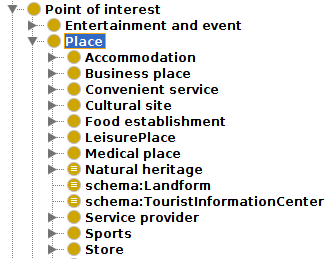
\includegraphics[scale=0.5]{ontology.png}
\caption{Subset of the modified version of the ontology DATATourisme
%(http://info.datatourisme.gouv.fr/ontology/core/2.0/)
}
\label{fig:ontology}
\end{figure}

The high level classes that are directly linked to the context factors are:
\begin{itemize}
    \item \textit{Museum}
    \item \textit{Interpretation Center}
    \item \textit{Library}
    \item \textit{Park and Garden}
    \item \textit{Archaeological Site}
    \item \textit{Religious Site}
    \item \textit{Remarkable Building}
    \item \textit{City Heritage}
    \item \textit{Defense Site}
    \item \textit{Remembrance Site}
    \item \textit{Technical Heritage}
    \item \textit{Food Establishment}
    \item \textit{Natural Heritage}
    \item \textit{Sports}
    \item \textit{Leisure Place}
    \item \textit{Store}
\end{itemize}

%\subsection{Relevances}
\subsection{From real users to simulated scenarios}
\label{section:relevances-survey}

In order to test several scenarios with different user's preferences, profiles, and behaviors,  we created synthetic scenarios, however based on data gathered from real people.
We asked people to fill a google form with two parts: 

\begin{enumerate}
    \item To determine the relevances for each context factor. The list of asked context factors included weather (with possible values {\tt rainy, cloudless, snowy}), time (with possible values {\tt wearly morning, morning, afternoon, night}) and day (with possible values {\tt weekday, weekend}). The list of asked types of POIs was the high level classes listed in the previous section. The question was "how much the context factor $c$ with value $v$ influences your decision to go to a 'place/event' of the type $t$ (these types are not exclusive)". People should answer an integer value between $0$ and $10$, where: 
\begin{itemize}
    \item $0$ means that if the context factor is met, you would not go to the place / event.
    \item 5 means you don't care if the context is met or not.
    \item 10 means that if the context is met, you would go to the place / event.
\end{itemize}

Then, Eq. (\ref{eq:avg}) is applied to each context factor, hence average them and transforming them to be on range $[0,2]$ by dividing by $5$.

\begin{equation}
    \label{eq:avg}
    AVG(contextfactor)/5
\end{equation}

 \item To determine users' preferences to tourism categories (i.e., classes of the POI ontology). In this part of the questionnaires, people provided their preferences  of high level ontology classes mentioned before, and also the genre, country, profession, age, and (optional) social networks to have more information for further work. 
 
 %The answer should be integers on range $[1, 10]$. Again, answers were more concentrated on the middle and highest options, but there were few low answers.
 
\end{enumerate}
    
    Both for relevance and preferences, we got around 100 answers from people of different ages, professions, and countries.  With this information a set of synthetic touris is generated, with different behaviors for different context scenarios.
    

%To define each $r_{c,x}$ for each node $c$ and context factor $x$, it was decided to gather real data provided by real people through a survey and then average them. The survey consisted of the question "Answer how much a 'context factor' influences your decision to go to a place/event of the specified type (these types are not exclusive)". Then, for each of the high level classes, people had to answer a real value between $0$ and $10$, where:
%\begin{itemize}
 %   \item $0$ means that if the context factor is met, you would not go to the place / event.
  %  \item 5 means you don't care if the context is met or not.
   % \item 10 means that if the context is met, you would go to the place / event.
%\end{itemize}

%Then the following formula is applied to each feature or column, hence average them and transforming them to be on range $[0,2]$:
% $$AVG(column)/5$$

%The form had a total of 34 answers. Something worth to mention was that the answers were concentrated between the options $0$, $5$ and $10$, maybe because it is easier to think something between the thoughts "I would not", "I don't care" and "I would", than to think something that is in the middle of two of those thoughts.

%\subsection{Users data}
%As explained before, a user of the system have to give initial preferences to some ontology classes. It was decided to make a form where people could answer their preferences of the high level ontology classes mentioned before. The form had a total of 63 answers. The genre, country, profession, age and (optional) social networks were also asked to have more information for further work. The answer should be integers on range $[1, 10]$. Again, answers were more concentrated on the middle and highest options, but there were few low answers.

\subsubsection{Simulated scenarios}
To evaluate the system, it was decided to test it with simulated scenarios (simulated contexts and simulated users). A set of centroids of a set of clusters were chosen as the set of simulated users from the user preferences gathered before. The \textit{K-Means} algorithm was used to get the clusters and the \textit{Elbow Method} (see Figure \ref{fig:elbow}) was used to choose $4$ as the number of clusters, since increasing this number does not make improvements worth the cost using our small dataset. In future work, a larger dataset should be used.

\begin{figure}[h]
    \centering
    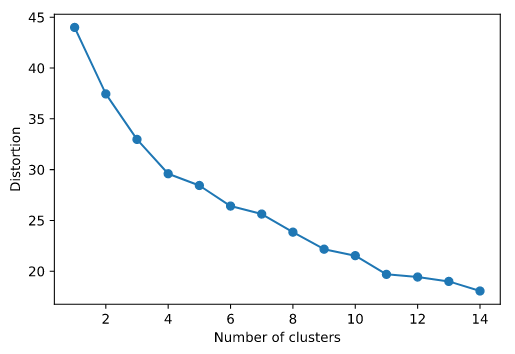
\includegraphics[scale=0.45]{elbow.png}
    \caption{Distortions of the different number of clusters}
    \label{fig:elbow}
\end{figure}

The centroids of four clusters represent our four synthetic tourists, $T_1, T_2, T_3, T_4$. Table \ref{table:centroids} shows the preferences for each tourist to each tourism category, according our light version of DATATourise ontology.  Figure \ref{fig:tourist_hist} shows how the initial preferences are distributed for each tourist.
%On figure \ref{fig:tourist_hist} we can see how are initial preferences distributed for each tourist.
\begin{table}[h!]
\centering
\caption{Centroids to be used as simulated users.}
\label{table:centroids}
\begin{tabular}{ |c|c|c|c|c| } 
    \hline
    Class & $T_1$ & $T_2$ & $T_3$ & $T_4$ \\
    \hline
    \hline

    Museum & 0.7235 & 0.6476 & 0.78 & 0.9421 \\ 
    \hline
    Interpretation Center & 0.6824 & 0.6476 & 0.52 & 0.8737 \\
    \hline
    Library & 0.5588 & 0.46667 & 0.72 & 0.7684 \\
    \hline
    Park and Garden & 0.865 & 0.8714 & 0.7 & 0.9316 \\
    \hline
    Archaeological Site & 0.6882 & 0.8619 & 0.82 & 0.826 \\
    \hline
    Religious Site & 0.45882 & 0.7 & 0.36 & 0.7316 \\
    \hline
    Remarkable Building & 0.6529 & 0.8524 & 0.4 & 0.7895 \\
    \hline
    City Heritage & 0.7412 & 0.919 & 0.58 & 0.8632 \\
    \hline
    Defence Site & 0.5412 & 0.8529 & 0.68 & 0.7421 \\
    \hline
    Remembrance Site & 0.4941 & 0.781 & 0.8 & 0.7211 \\
    \hline
    Technical Heritage & 0.4059 & 0.7905 & 0.56 & 0.5842 \\
    \hline
    Food Establishment & 0.9059 & 0.8905 & 0.7 & 0.6632 \\
    \hline
    Natural Heritage & 0.9059 & 0.9143 & 0.76 & 0.9211 \\
    \hline
    Sports & 0.9353 & 0.8429 & 0.22 & 0.6316 \\
    \hline
    Leisure Place & 0.9353 & 0.8429 & 0.22 & 0.6316 \\
    \hline
    Store & 0.7647 & 0.8286 & 0.28 & 0.5684 \\
    
    \hline
\end{tabular}
\end{table}

\begin{figure}[h]
    \centering
    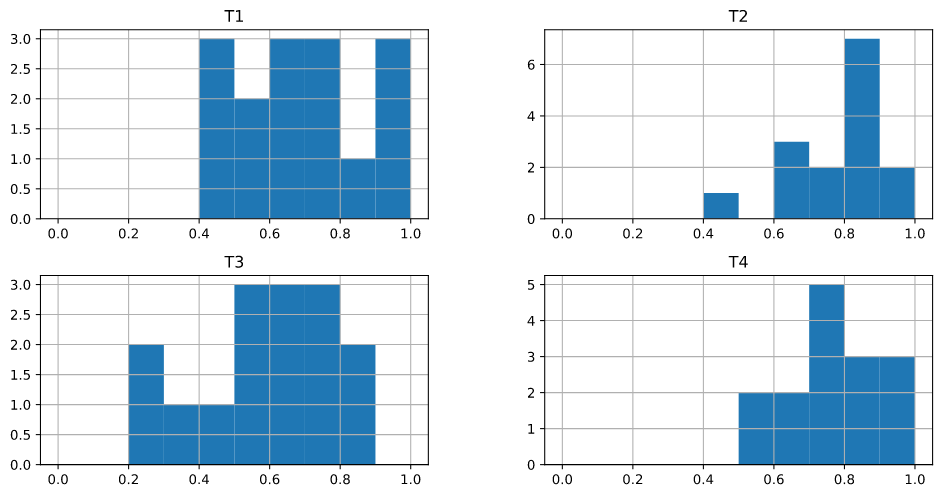
\includegraphics[scale=0.25]{tourist_histogram.png}
    \caption{Distributions of initial preferences of $T_1$, $T_2$, $T_3$ and $T_4$}
    \label{fig:tourist_hist} 
\end{figure}

For our experiments, the same relevances are shared between synthetic users, however future work should evaluate different relevances for each user tested. These relevances are shown on table \ref{table:relevances-experiment}.

\begin{table*}[h!]
\centering
\caption{Centroids to be used as simulated users.}
\label{table:relevances-experiment}
\begin{tabular}{ |c|c|c|c|c|c|c|c|c|c| } 
    \hline
    \textbf{Class} & \textbf{rainy} & \textbf{cloudless} & \textbf{snowy} & \textbf{workday} & \textbf{weekend} & \textbf{morning} & \textbf{afternoon} & \textbf{night} & \textbf{early morning} \\
    \hline
    \hline

    Museum & 1.0 & 1.394 & 1.029 & 1.082 & 1.488 & 1.065 & 1.518 & 0.788 & 0.194 \\ \hline
    
    Interpretation Centre & 0.871 & 1.312 & 0.829 & 1.029 & 1.424 & 1.029  & 1.382 & 0.771 & 0.135 \\ \hline

    Libreary & 1.271 & 1.388  & 1.188  & 1.312 &1.159 & 1.324 & 1.453 & 0.729  & 0.271 \\ \hline

    Park and garden &
    0.335 & 1.847  & 0.894 & 1.365 & 1.665 & 1.388  & 1.629 & 0.924 & 0.494  \\ \hline

    Archeological Site &
    0.476 & 1.488 & 0.671 & 0.782 & 1.471 & 1.235 & 1.424 & 0.682  & 0.335 \\ \hline

    Religious Site &
    0.8 & 1.018 & 0.841  & 0.641  & 1.106 & 1.018 & 0.971 & 0.529  & 0.1 \\ \hline

    Remarkable building &
    0.912 & 1.576  & 0.994  & 1.165 & 1.506 & 1.241  & 1.453 & 1.0056 & 0.324 \\ \hline
    
    City heritage &
    0.665 & 1.629  & 0.947  & 1.088  & 1.618 & 1.329  & 1.565 & 1.271 & 0.5 \\ \hline
    
    Defense Site &
    0.712 & 1.412 & 0.806 & 0.835  & 1.376  & 1.253 & 1.388  & 0.824 & 0.265 \\ \hline
    
    Remembrance Site &
    0.588  & 1.318 & 0.812 & 0.935  & 1.306 & 1.129  & 1.294  & 0.6 & 0.324 \\ \hline
    
    Technical Heritage &
    0.582  & 1.371 & 0.682  & 0.841  & 1.3 & 1.265 & 1.3 & 0.741  & 0.3 \\ \hline
    
    Food Stablishment &
    1.488  & 1.624 & 1.494  & 1.635  & 1.759 & 1.353 & 1.671 & 1.676  & 0.688  \\ \hline
    
    Natural Heritage &
    0.494  & 1.776 & 0.835  & 1.088  & 1.659 & 1.535  & 1.524 & 0.953 & 0.465 \\ \hline
    
    Leisure place &
    1.088  & 1.541  & 1.006 & 1.118 & 1.588  & 1.024 & 1.506 & 1.418 & 0.588  \\ \hline
    
    Sports &
    0.1 & 2.0 & 0.75 & 1.118 & 1.588  & 1.024 & 1.506 & 0.8 & 0.588  \\ \hline
    
    Store &
    1.312 & 1.535  & 1.241  & 1.388  & 1.435  &1.0588  & 1.547  & 1.1647  & 0.3 \\ \hline


\end{tabular}
\end{table*}

\subsection{Metrics} \label{section:metrics}
For each centroid of the clusters mentioned previously, we simulate two visits to Niza, Lyon, and Paris for each possible context using each possible value for each context factor \textcolor{red}{Se podría poner esto en una tablita para verlo más fácilmente, quizás por $T_i$?}. The system returns a set of not more than $5$ recommended places inside a radius of $8$ kilometers for each visit, this set is going to be called the \textit{recommendation}. Let $R$ be a recommendation for a specific user on a specific location and a specific context, we define the following recommendation metrics:
\begin{equation}
    pref_{R} = \frac{ \displaystyle \sum_{p \in R}{pref_p} }{| R |}
\end{equation}

\begin{equation}
    act_{R} = \frac{ \displaystyle \sum_{p \in R}{act_p} }{| R |}
\end{equation}

\begin{equation}
    \eta_{R} = \frac{ \displaystyle \sum_{p \in R}{\eta_p} }{| R |}
\end{equation}

\begin{equation}
    dist_{u, R} = \frac{ \displaystyle \sum_{p \in R}{dist_{u, p}} }{| R |}
\end{equation}

To compute novelty \cite{kotkov2016survey} we use the following metric:
\begin{equation} \label{eq:novelty}
    nov_{u, p} = \  \underaccent{q \in rec(u)}{min} \  ( dist( c_p, c_q ) )
\end{equation}
where $p$ is a recommended place, $u$ the user to which $p$ was recommended, $rec(u)$ is the set of already recommended places to $u$, $c_p$ is the ontology class to which $p$ belongs and $dist$ computes the distance in the ontology (using \textit{Breadth First Search}) of two ontology classes. Finally, the system returns the average of each recommendation metric.

Now we can define the novelty of a recommendation as follows:
\begin{equation}
    nov_{u, R} = \frac{ \displaystyle \sum_{p \in R}{nov_{u, p}} }{| R |}
\end{equation}

\subsection{Experiments} \label{section:experiments}
We use different coefficients for the score (see Section \ref{section:score}), and since we said $maxdist$ is $8$ for these experiments, we are ignoring it as argument. 

\subsubsection{First configuration} \label{section:experiment-1}
First we consider $k_1 = \frac{1}{4} + \frac{1}{9}$ for preference, $k_2 = \frac{1}{4} + \frac{1}{9}$ for activation, $k_3 = \frac{1}{4}$ for aging and $k_4 = \frac{1}{4} - \frac{2}{9}$ for distance from user, resulting on equation \ref{eq:score-1} and giving more priority to preference and activation and very little priority to distance from user. With these parameters we start simulating each user and their visits.
\begin{equation} \label{eq:score-1}
    \begin{split}
        score_p = \ &\frac{13}{36} \cdot pref_c + \frac{13}{36} \cdot act_c \\
                                        &+ \frac{1}{4} \cdot \eta_p - \frac{1}{36} \cdot \frac{dist_{u,p}}{8}
    \end{split}
\end{equation}


\textcolor{red}{Hace falta una tablita que muestre los contextos y las preferencias de cada Ti , y quizás también el weather real y la configuración (por configuración).
Y en las tablas de recommendaciones poner pi (el sitio) y Quizás para que no hayan tantas tablas se puede hacer solo una con todas las visitas por turista y mostrar los 4 turistas. Podemos habla para decidir cómo irían las tablas.}

We are showing some sets of recommended items like table \ref{table:t1-1}, where each $p_i$ is a recommended place and $score_{p_i} \ge score_{p_j}$ for every $i < j$. Table \ref{table:t1-1} corresponds to $T_1$'s first visit to Niza, on a rainy workday in the morning, where $p_1$ is Train des Merveilles (from class \textit{TouristTrain}), $p_2$ is Cinéma de Plein Air (from class \textit{Cinema}), $p_3$ is Casino de Beaulieu (from class \textit{Casino}), $p_4$ is Cinéma de Beaulieu (from class \textit{Cinema}) and $p_5$ is Lyon-style petanque fields (from class \textit{BoulesPitch}). We can see that since each of the places' ontology classes are subclasses of \textit{LeisurePlace}, which $T_1$ loves, they have same preference and activation and since this is the first recommendation, all aging values are $1.0$. Therefore, the distance is the tiebreaker. Despite of a rainy morning, the system recommends a tourist train to $T_1$, just because it is a leisure place.
\begin{table}[h!]
    \centering
    \begin{tabular}{ |c|c|c|c|c|c| } 
        \hline
        Field   & $p_1$ & $p_2$ & $p_3$ & $p_4$ & $p_5$ \\
        \hline
        $pref_c$    &  0.9353 & 0.9353 & 0.9353 & 0.9353 & 0.9353 \\
        $act_c$     & 4.4 & 4.4 & 4.4 & 4.4 & 4.4 \\
        $\eta_p$    & 1.0 & 1.0 & 1.0 & 1.0 & 1.0 \\
        $dist_{u,p}$ & 1.53 & 3.99 & 5.52 & 5.53 & 5.58 \\
        $score_p$    & 2.1713 & 2.1628 & 2.15745 & 2.15742 & 2.1573 \\
        
        \hline
    \end{tabular}
    \caption{First visit of $T_1$ to Niza with first configuration}
    \label{table:t1-1}
\end{table}


At the second visit to Lyon (see table \ref{table:t1-3}), on a rainy workday in the morning, only $p_1$ is not a leisure place but an interpretation center, a kind of place $T_1$ does not like as much as leisure places. However, the activation of \textit{InterpretationCenter} is higher enough to make $score_{p_1}$ greater than $score_{p_2}$. Despite of $p_1$ being very far away from $T_1$'s location, the little magnitude of $k_4$ makes it little important to the final score. Something odd on the recommended set is that $p_3$ and $p_4$ are the same place, Le Sucre, but reported as belonging to two different ontology classes: \textit{NightClub} and \textit{Theatre}, respectively.

\begin{table}[h!]
    \centering
    \begin{tabular}{ |c|c|c|c|c|c| } 
        \hline
        Field   & $p_1$ & $p_2$ & $p_3$ & $p_4$ & $p_5$ \\
        \hline
        $pref_c$    & 0.676 & 0.9353 & 0.9353 & 0.9353 & 0.9353 \\
        $act_c$     & 4.818 & 4.51 & 4.51 & 4.51 & 4.51 \\
        $\eta_p$    & 1.0 & 1.0 & 1.0 & 1.0 & 1.0 \\
        $dist_{u,p}$ & 7.1 & 4.45 & 4.54 & 4.54 & 4.61 \\
        $score_p$    & 2.2092 & 2.2015 & 2.2012 & 2.2012 & 2.2010 \\
        
        \hline
    \end{tabular}
    \caption{Second visit of $T_1$ to Lyon with first configuration}
    \label{table:t1-3}
\end{table}

At the fourth visit to Niza, on a rainy workday in the early morning, the system recommends table \ref{table:t1-2} to $T_1$, where $p_1$ is Cinéma de Plein Air (from class \textit{Cinema}), $p_2$ is Ferronnerie d'art JC Rodriguez (from class \textit{CraftsmanShop}), $p_3$ is Atelier Hesperida (from class \textit{CraftsmanShop}), $p_4$ is Horlogerie Foltête	(from class \textit{CraftsmanShop}) and $p_5$ is Galerie Bizet (from class \textit{CraftsmanShop}). Since $T_1$ loves leisure places more than stores, the predicted preference for Cinéma de Plein Air is greater than the other ones on this visit. However, we can see that $\eta_{p_1}$ lowers down $score_{p_1}$ to a value not so different from $score_{p_2}$. Cinéma de Plein Air does not appear again before a snowy workday afternoon, due to its aging and the $T_1$'s context.

\begin{table}[h!]
    \centering
    \begin{tabular}{ |c|c|c|c|c|c| } 
        \hline
        Field   & $p_1$ & $p_2$ & $p_3$ & $p_4$ & $p_5$ \\
        \hline
        $pref_c$    &  0.9353 & 0.7647 & 0.7647 & 0.7647 & 0.7647 \\
        $act_c$     & 4.2 & 4.1 & 4.1 & 4.1 & 4.1 \\
        $\eta_p$    & 0.6 & 1.0 & 1.0 & 1.0 & 1.0 \\
        $dist_{u,p}$ & 3.99 & 5.21 & 5.25 & 5.72 & 5.737 \\
        $score_p$    & 1.9906 & 1.9886 & 1.9884 & 1.98684 & 1.98678 \\
        
        \hline
    \end{tabular}
    \caption{Fourth visit of $T_1$ to Niza with first configuration}
    \label{table:t1-2}
\end{table}

While the system recommends same places to $T_1$ and $T_2$ for their first visits to Niza, Lyon and Paris, at rainy workdays at afternoon, the sets start to diverge after the second visits. The system recommends to $T_1$ a set of leisure places and one interpretation center for the second visit to Lyon, but recommends a set with two archeological sites, one interpretation center and two remarkable buildings to $T_2$, in that order (see table \ref{table:t2-1}). The more diverse initial preferences of $T_2$ and the aging system are responsible for this.

\begin{table}[h!]
    \centering
    \begin{tabular}{ |c|c|c|c|c|c| } 
        \hline
        Field   & $p_1$ & $p_2$ & $p_3$ & $p_4$ & $p_5$ \\
        \hline
        $pref_c$    &  0.852 & 0.852 & 0.659 & 0.843 & 0.843 \\
        $act_c$     & 4.659 & 4.659 & 4.818 & 4.6 & 4.6 \\
        $\eta_p$    & 1.0 & 1.0 & 1.0 & 1.0 & 1.0 \\
        $dist_{u,p}$ & 3.967 & 5.267 & 7.0969 & 3.967 & 5.267 \\
        $score_p$    & 2.226 & 2.222 & 2.203 & 2.202 & 2.197 \\
        
        \hline
    \end{tabular}
    \caption{Second visit of $T_2$ to Lyon with first configuration}
    \label{table:t2-1}
\end{table}

After many visits, again at a rainy workday at afternoon, the system recommends a completely different set of places to $T_2$ when visiting Lyon again. It recommends a theater, an art gallery, a craftsman shop and two other art galleries, in that order (see table \ref{table:t2-2}). The system aging is responsible for this variety of recommendations.
\begin{table}[h!]
    \centering
    \begin{tabular}{ |c|c|c|c|c|c| } 
        \hline
        Field   & $p_1$ & $p_2$ & $p_3$ & $p_4$ & $p_5$ \\
        \hline
        $pref_c$    &  0.843 & 0.829 & 0.829 & 0.829 & 0.829 \\
        $act_c$     & 4.512 & 4.371 & 4.371 & 4.371 & 4.371 \\
        $\eta_p$    & 0.8 & 1.0 & 1.0 & 1.0 & 1.0 \\
        $dist_{u,p}$ & 7.157 & 5.425 & 5.438 & 5.442 & 5.462 \\
        $score_p$    & 2.10876 & 2.10864 & 2.10859 & 2.10858 & 2.10851 \\
        
        \hline
    \end{tabular}
    \caption{A visit of $T_2$ to Lyon with first configuration after many visits}
    \label{table:t2-2}
\end{table}

However, there are cases where $k_3$ is not high enough to make more diverse the recommendations, as in the two visits of $T_2$ to Paris on cloudless workdays at early morning (see tables \ref{table:t2-3} and \ref{table:t2-4}), where the second one is made after many visits. Both visits involve Garnier Opera (from class \textit{Palace}), Conciergerie (from class \textit{Palace}) and Le Manoir de Paris (from class \textit{InterpretationCentre}), as $p_2$, $p_3$ and $p_4$ for the first visit and $p_1$, $p_5$ and $p_2$ for the second visit, respectively.

\begin{table}[h!]
    \centering
    \begin{tabular}{ |c|c|c|c|c|c| } 
        \hline
        Field   & $p_1$ & $p_2$ & $p_3$ & $p_4$ & $p_5$ \\
        \hline
        $pref_c$    &  0.829 & 0.843 & 0.843 & 0.659 & 0.659 \\
        $act_c$     & 4.171 & 4.4 & 4.4 & 4.571 & 4.571 \\
        $\eta_p$    & 0.8 & 0.4 & 0.4 & 0.4 & 0.4 \\
        $dist_{u,p}$ & 7.51 & 4.25 & 5.06 & 5.9 & 6.3 \\
        $score_p$    & 1.97916 & 1.97869 & 1.97590 & 1.96803 & 1.96665 \\
        
        \hline
    \end{tabular}
    \caption{First visit of $T_2$ to Paris with first configuration on a cloudless workday at early morning}
    \label{table:t2-3}
\end{table}

\begin{table}[h!]
    \centering
    \begin{tabular}{ |c|c|c|c|c|c| } 
        \hline
        Field   & $p_1$ & $p_2$ & $p_3$ & $p_4$ & $p_5$ \\
        \hline
        $pref_c$    &  0.843 & 0.843 & 0.659 & 0.659 & 0.659 \\
        $act_c$     & 4.40 & 4.40 & 4.57 & 4.57 & 4.57  \\
        $\eta_p$    & 0.4 & 0.4 & 0.4 & 0.4 & 0.4 \\
        $dist_{u,p}$ & 4.25 & 5.06 & 3.79 & 4.55 & 5.9 \\
        $score_p$    & 1.97869 & 1.97590 & 1.97535 & 1.97273 & 1.96803 \\
        
        \hline
    \end{tabular}
    \caption{Second visit of $T_2$ to Paris with first configuration on a cloudless workday at early morning}
    \label{table:t2-4}
\end{table}

Table \ref{table:config-1} shows the average of the recommendation metrics for each tourist using first configuration. Averages of $pref_R$ of $T_1$'s and $T_2$'s visits are the highest ones, being greater than $0.8$ and hence closer to $1.0$, the maximum possible value. Next is $T_4$'s, being greater than $0.7$, which is still a good average preference. $T_3$'s average $pref_R$ is lower, but we can blame the amount of low initial preferences of $T_3$, as we can see on figure \ref{fig:tourist_hist}.
\begin{table}[h!]
    \centering
    \begin{tabular}{ |c|c|c|c|c| } 
        \hline
        avg & $T_1$ & $T_2$ & $T_3$ & $T_4$ \\
        \hline
        \hline
        $avg(pref_R)$ & 0.8555 & 0.8213 & 0.4183 & 0.7269\\
        $avg(act_R)$ & 4.286 & 4.3092 & 4.314 & 4.3319 \\
        $avg(\eta_R)$ & 0.7058 & 0.7111 & 0.6906 & 0.6914 \\
        $avg(nov_{u,R})$ & 0.0923 & 0.1231 & 0.1329 & 0.1147 \\
        $avg(dist_{u,R})$ & 4.876 & 4.8993 & 4.9101 & 4.9861 \\
       
        \hline
    \end{tabular}
    \caption{Averages of recommendations metrics with first configuration}
    \label{table:config-1}
\end{table}

The average $act_R$ of each tourist is greater than $4.0$. Theoretically, the maximum possible value is $6.0$, but since the relevance values obtained by the survey (see section \ref{section:relevances-survey}) do not reach their maximum possible value, which is $2.0$, it is impossible for these experiments.

Average $\eta_R$ is very near $0.7$, hence the amount of "young" recommended places is high. Theoretically, the maximum possible value is $1.0$, but that would be possible if each recommendation involves POIs never recommended before. 

Despite of recommending places with distance from user near $8.0$ km, the average $dist_{u,R}$ for each tourist is acceptable: greater than $4.0$ km and less than $5.0$ km. The novelties measured as we proposed on section \ref{section:metrics} have bad performance on four tourists.

\subsubsection{Second configuration} \label{section:experiment-2}
Now we consider $k_1 = \frac{1}{4}$ for preference, $k_2 = \frac{1}{4}$ for activation, $k_3 = \frac{1}{4} + \frac{2}{9}$ for aging and $k_4 = \frac{1}{4} - \frac{2}{9}$ for distance from user, resulting on equation \ref{eq:score-2} and giving now more priority to aging.
\begin{equation} \label{eq:score-2}
    \begin{split}
        score_p = \ &\frac{1}{4} \cdot pref_c + \frac{1}{4} \cdot act_c \\
                                        &+ \frac{17}{36} \cdot \eta_p - \frac{1}{36} \cdot \frac{dist_{u,p}}{8}
    \end{split}
\end{equation}

For the first visit of $T_1$ to Niza in a cloudless workday at afternoon, the $\eta_R$ is $0.84$ using the second configuration (see table \ref{table:2nd-t1-niza-1}), while it is $0.80$ using the first configuration (see table \ref{table:1st-t1-niza-1}). Even the $pref_R$ improve, from $0.765$ to $0.799$, but the $act_R$ goes from $4.44$ to $4.33$.

\begin{table}[h!]
    \centering
    \begin{tabular}{ |c|c|c|c|c|c| } 
        \hline
        Field   & $p_1$ & $p_2$ & $p_3$ & $p_4$ & $p_5$ \\
        \hline
        $pref_c$    &  0.76 & 0.76 & 0.76 & 0.76 & 0.76 \\
        $act_c$     & 4.44 & 4.44 & 4.44 & 4.44 & 4.44  \\
        $\eta_p$    & 0.8 & 0.8 & 0.8 & 0.8 & 0.8 \\
        $dist_{u,p}$ & 5.25 & 5.72 & 5.74 & 5.78 & 5.79 \\
        $score_p$    & 2.06166 & 2.06004 & 2.05998 & 2.05983 & 2.05981 \\
        
        \hline
    \end{tabular}
    \caption{First visit of $T_1$ to Niza with first configuration on a cloudless workday at afternoon}
    \label{table:1st-t1-niza-1}
\end{table}

\begin{table}[h!]
    \centering
    \begin{tabular}{ |c|c|c|c|c|c| } 
        \hline
        Field   & $p_1$ & $p_2$ & $p_3$ & $p_4$ & $p_5$ \\
        \hline
        $pref_c$    &  0.76 & 0.76 & 0.935 & 0.76 & 0.76 \\
        $act_c$     & 4.44 & 4.44 & 3.89 & 4.44 & 4.44  \\
        $\eta_p$    & 0.8 & 0.8 & 1.0 & 0.8 & 0.8 \\
        $dist_{u,p}$ & 5.20 & 5.25 & 5.30 & 5.72 & 5.73 \\
        $score_p$    & 1.6612 & 1.6610 & 1.6597 & 1.6594 & 1.6593 \\
        
        \hline
    \end{tabular}
    \caption{First visit of $T_1$ to Niza with second configuration on a cloudless workday at afternoon}
    \label{table:2nd-t1-niza-1}
\end{table}

For the second visit of $T_4$ to Paris on a snowy weekend at early morning, the $\eta_R$ is $0.774$ using second configuration (see table \ref{table:1st-t4-Paris-2}), while it is $0.691$ using first configuration (see table \ref{table:2nd-t4-Paris-2}). The $pref_R$ and the $act_R$ decrease from $0.727$ to $0.699$ and from $4.332$ to $4.041$, respectively.

\begin{table}[h!]
    \centering
    \begin{tabular}{ |c|c|c|c|c|c| } 
        \hline
        Field   & $p_1$ & $p_2$ & $p_3$ & $p_4$ & $p_5$ \\
        \hline
        $pref_c$    &  0.866 & 0.866 & 0.790 & 0.866 & 0.866 \\
        $act_c$     & 4.288 & 4.288 & 4.265 & 4.288 & 4.288  \\
        $\eta_p$    & 0.4 & 0.4 & 0.4 & 0.2 & 0.2 \\
        $dist_{u,p}$ & 5.899 & 6.297 & 4.253 & 3.791 & 4.546 \\
        $score_p$    & 1.941 & 1.939 & 1.911 & 1.898 & 1.895 \\
        
        \hline
    \end{tabular}
    \caption{Second visit of $T_4$ to Paris with first configuration on a snowy weekend at early morning}
    \label{table:1st-t4-Paris-2}
\end{table}

\begin{table}[h!]
    \centering
    \begin{tabular}{ |c|c|c|c|c|c| } 
        \hline
        Field   & $p_1$ & $p_2$ & $p_3$ & $p_4$ & $p_5$ \\
        \hline
        $pref_c$    &  0.866 & 0.866 & 0.738 & 0.866 & 0.866 \\
        $act_c$     & 4.288 & 4.288 & 3.81 & 4.288 & 4.288  \\
        $\eta_p$    & 1.0 & 1.0 & 0.6 & 0.2 & 0.2 \\
        $dist_{u,p}$ & 3.791 & 4.546 & 5.333 & 5.899 & 6.297 \\
        $score_p$    & 1.748 & 1.745 & 1.402 & 1.363 & 1.361 \\
        
        \hline
    \end{tabular}
    \caption{Second visit of $T_4$ to Paris with second configuration on a snowy weekend at early morning}
    \label{table:2nd-t4-Paris-2}
\end{table}

Table \ref{table:config-2} shows the average of the recommendation metrics for each tourist using second configuration. Again, $T_1$'s and $T_2$'s $avg(pref_R)$ are the highest ones, followed by $T_4$'s, while $T_3$'s is the lowest. We can notice that only $T_1$'s and $T_2$'s $avg(pref_R)$ increase a little from the ones with first configuration, but the other two decrease. Again, all $avg(act_R)$ are above $4.0$, but each one decreases from the first configuration version. As expected, all $avg(\eta_R)$ increase because the second configuration gives more weight to aging.

\begin{table}[h!]
    \centering
    \begin{tabular}{ |c|c|c|c|c| } 
        \hline
        avg & $T_1$ & $T_2$ & $T_3$ & $T_4$ \\
        \hline
        \hline
        $avg(pref_R)$ & 0.8658 & 0.8272 & 0.3912 & 0.6987 \\
        $avg(act_R)$ & 4.0738 & 4.0818 & 4.0031 & 4.0415 \\
        $avg(\eta_R)$ & 0.7592 & 0.7619 & 0.7850 & 0.7739 \\
        $avg(nov_{u,R})$ & 0.172 & 0.1860 & 0.1986 & 0.1580 \\
        $avg(dist_{u,R})$ & 4.842 & 5.0215 & 4.8999 & 4.9615 \\
       
        \hline
    \end{tabular}
    \caption{Averages of recommendations metrics with second configuration}
    \label{table:config-2}
\end{table}


\section{Conclusions and future work}



%\medskip
 
 \bibliographystyle{unsrt}
 \balance
\bibliography{bibliography}
%\printbibliography

\end{document}
